% --------------------------------------------------------------------------- %
% Author:          Joey Dumont                <joey.dumont@gmail.com>         %
% Date created:    Jun 19th, 2015                                             %
% Date modified:   Jun 19th, 2015                                             %
% Description:     Prepared for IHPCSS 2015.                                  %
%                  TikZ code to show the DomainDecomposition method.          %
% License:         CC0                                                        %
%                  <https://creativecommons.org/publicdomain/zero/1.0>        %
% --------------------------------------------------------------------------- %

\documentclass[tikz]{standalone}
\usepackage[charter]{mathdesign}
\usepackage{amsmath}
\usepackage{xifthen}
\usepackage{fontspec}
\setmainfont{Oswald}
\usetikzlibrary{calc}

\newcommand{\focal}{5}
\newcommand{\parabola}[1]{\pgfmathsetmacro{\myvalue}{#1*#1/(4*\focal)-\focal}}
\newcommand{\iparabola}[1]{\pgfmathsetmacro{\myivalue}{sqrt(4*\focal*(#1+\focal))}}
\newcommand{\gaussian}[1]{\pgfmathsetmacro{\mygaussian}{exp(-pow(x/0.5,2)}}
\begin{document}

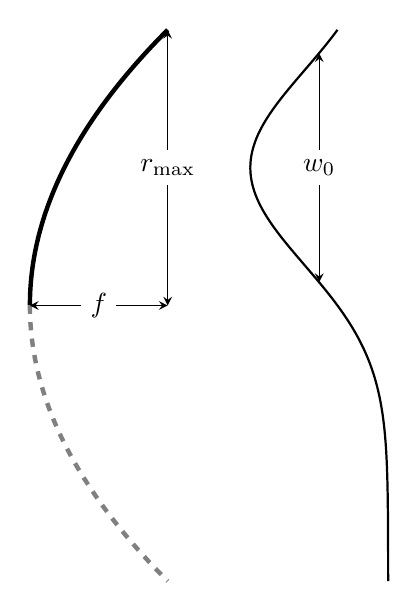
\begin{tikzpicture}[scale=0.35]
  \draw[domain=-\focal:0,samples=1000,ultra thick] plot (\x,{sqrt(4*\focal*(\x+\focal))});
  \draw[domain=-\focal:0,samples=1000,ultra thick,gray,dashed] plot (\x,{-sqrt(4*\focal*(\x+\focal))});

  \draw[<->,>=stealth] (-\focal,0) -- (0,0)         node[midway,fill=white] {$f$};
  \draw[<->,>=stealth] (0, 0)      -- (0,2*\focal)   node[midway,fill=white] {$r_\text{max}$};

  \begin{scope}[rotate=90,yshift=-8cm]
    \draw[domain=-10:10,samples=1000,thick] plot (\x,{5*exp(-pow((\x-\focal)/5,2))});
    \draw[<->,>=stealth] ($(-4.15, 2.5)+(\focal,0)$) -- ($(4.15, 2.5)+(\focal,0)$) node[midway,fill=white] {$w_0$};
  \end{scope}

\end{tikzpicture}

\end{document}